\begin{chapter}{\label{cha:wake}Classical-like wakes behind elliptical obstacles in Bose-Einstein condensates}

\section{Introduction}
\begin{figure}[!ht]
\centering
  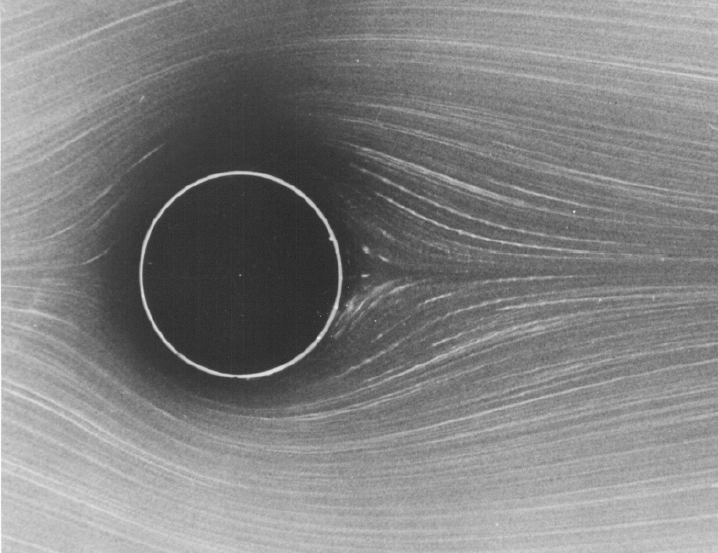
\includegraphics[height=2.08cm,angle=180]{wake/3.png}
  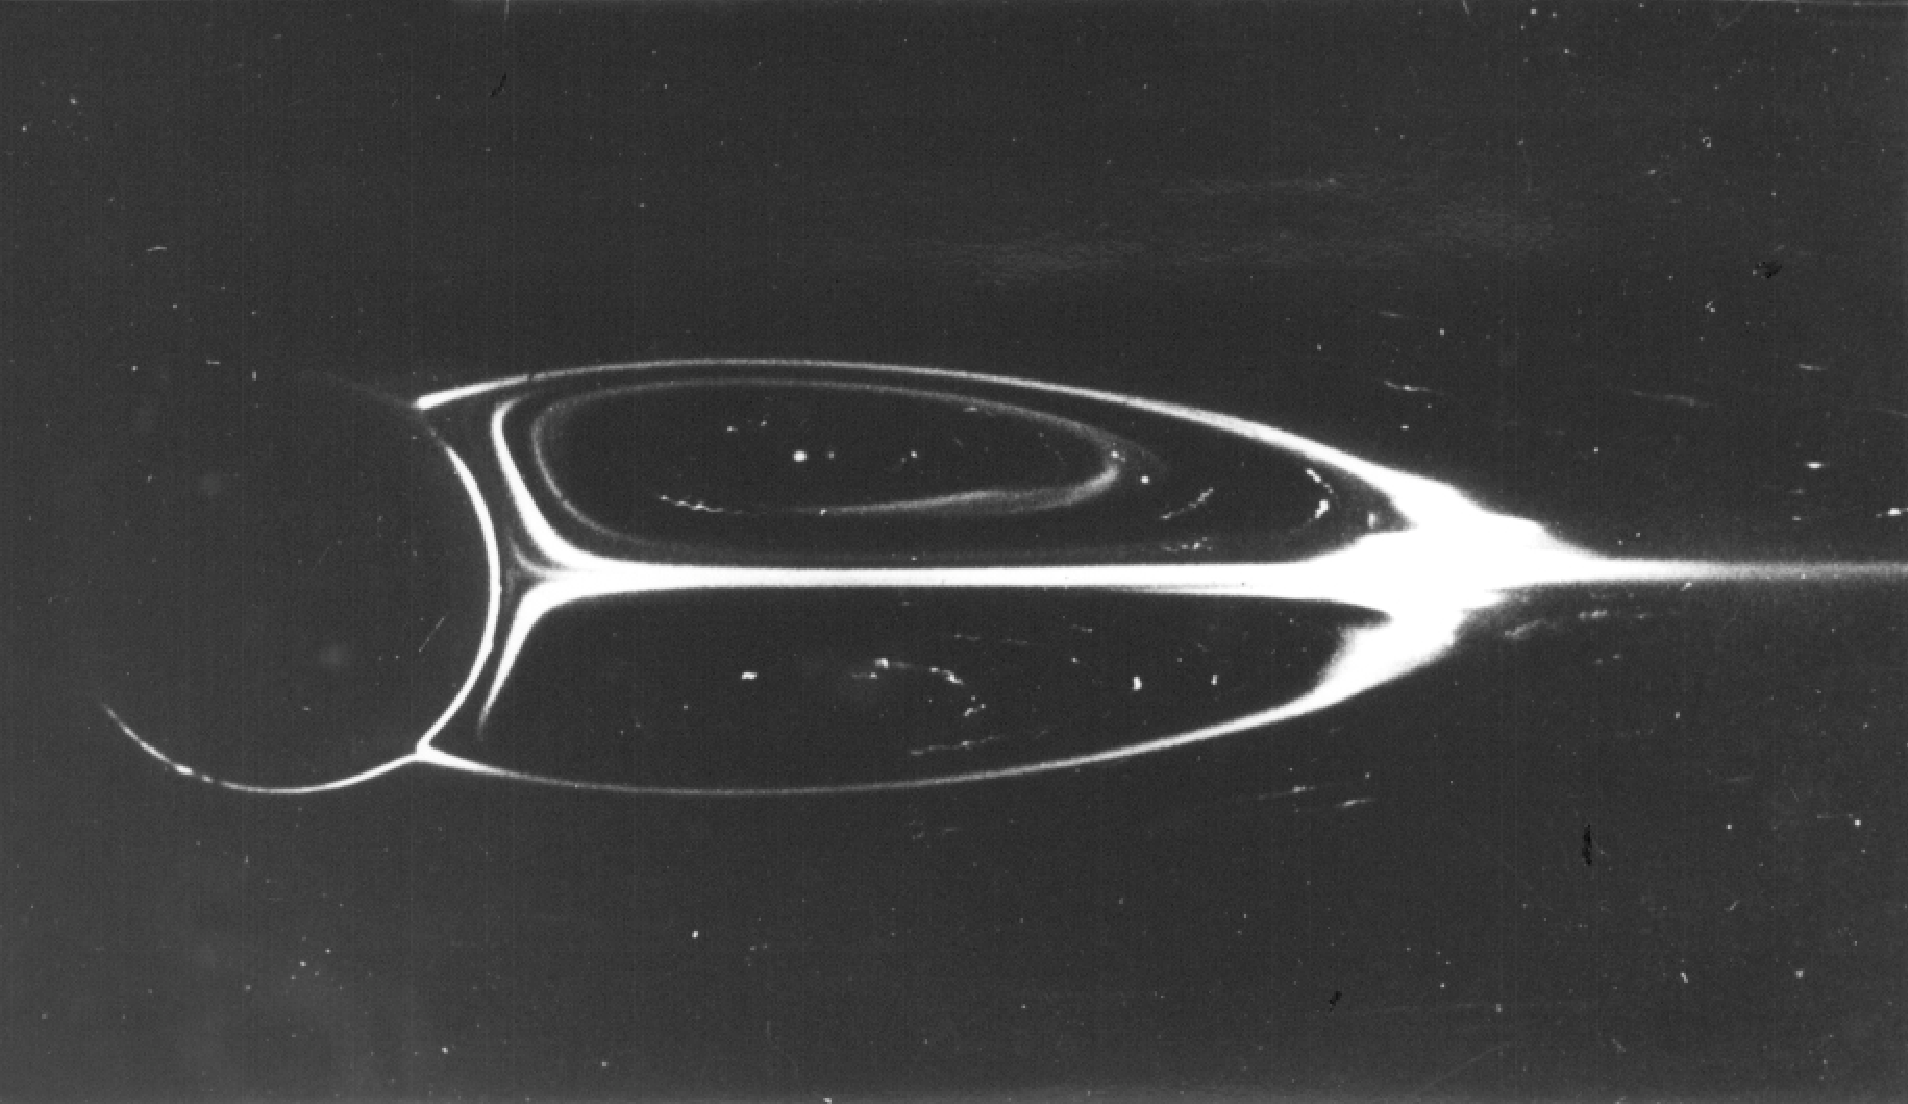
\includegraphics[width=0.24\textwidth,angle=180]{wake/taneda41}
  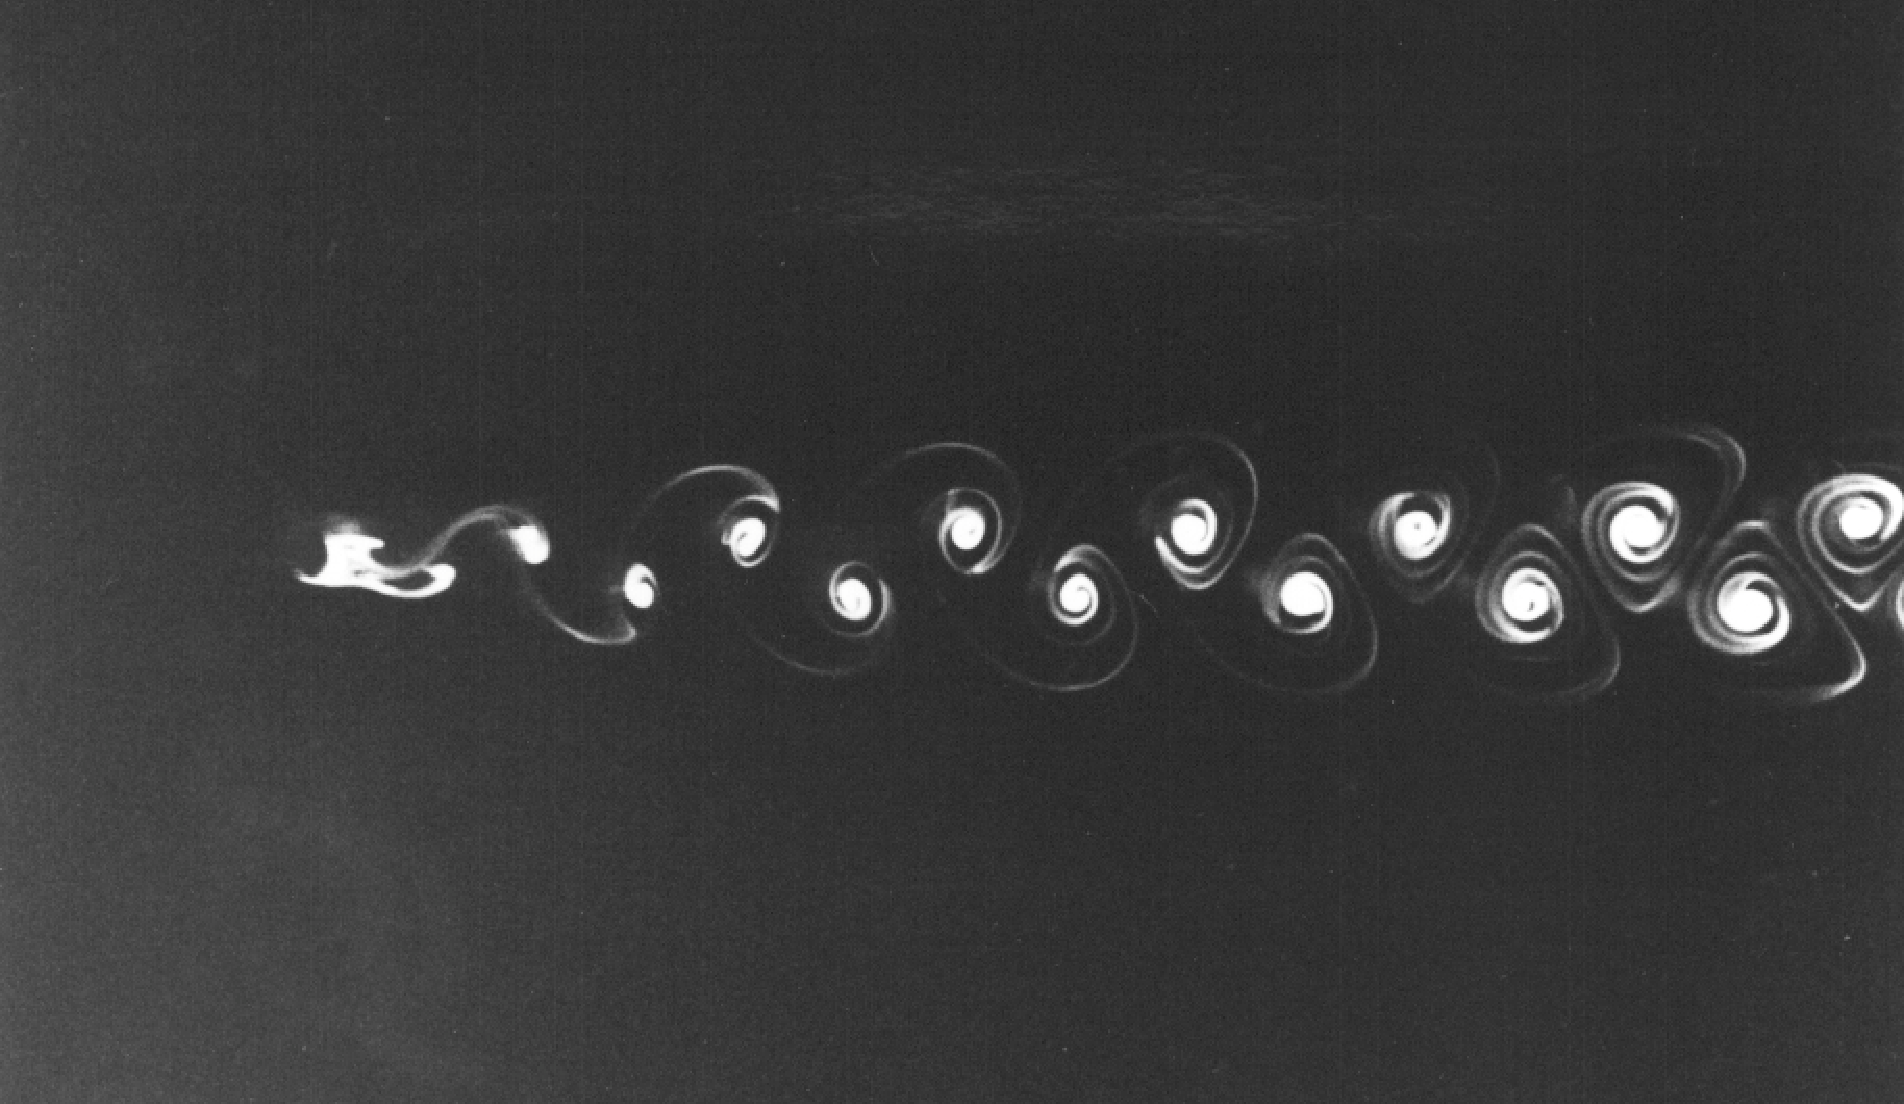
\includegraphics[width=0.24\textwidth,angle=180]{wake/taneda112}
    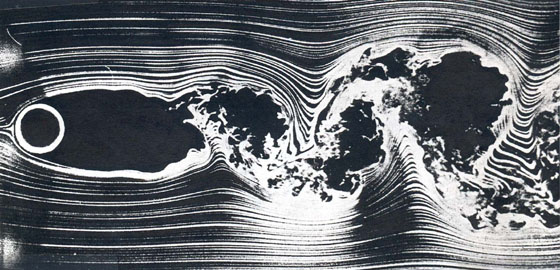
\includegraphics[width=0.29\textwidth,angle=180]{wake/turb.jpg}
  \caption{Classical viscous flow past a cylinder. From left to right: laminar flow ($\Rey=3.64$) \cite{taneda41}; steady symmetric wake behind the cylinder ($\Rey=41$) \cite{taneda41}; time-dependent B\'enard--von K\'arm\'an vortex street ($\Rey = 112$) \cite{taneda112}; and chaotic downstream wake ($\Rey > 10^5$) \cite{nagib}.} 
  \label{fig:taneda-imgs}
\end{figure}
Recent experimental \cite{Tabeling,Salort}, 
numerical \cite{Nore,Kobayashi,Laurie} 
and theoretical studies \cite{Lvov}
have highlighted similarities between turbulence in quantum
fluids and turbulence in ordinary (classical) fluids \cite{Frisch}.
In particular, it is found that, in
the idealized case of homogeneous isotropic conditions away from
boundaries, the distribution of kinetic energy over the 
length scales obeys the celebrated Kolmogorov scaling of 
classical turbulence \cite{barenghi}. This similarity is remarkable,
because a superfluid has zero viscosity and vorticity is not a continuous
field. In the more realistic presence of boundaries such as an obstacle or confining channel
walls, superfluid hydrodynamics is less understood, despite the large number of experiments in such scenarios. 

In a classical viscous fluid \cite{Frisch}, the prototype problem with
a boundary is the flow 
around a cylinder or a sphere (or, changing the frame of reference, 
the motion of a cylinder or a sphere in a fluid at rest).
The nature of such flow is determined by the Reynolds 
number $\Rey = vd/\nu$, where $v$ is the (assumed uniform)
flow's velocity away from the obstacle, $d$ is the obstacle's size,
and $\nu$ is the fluid's
kinematic viscosity. If $\Rey\lesssim50$, a steady symmetric 
wake forms behind the obstacle; if $10^2\lesssim\Rey\lesssim10^5$ the wake 
becomes asymmetric and time dependent, forming the famous 
B\'enard--von K\'arm\'an vortex street structure. For even higher values of $\Rey$,
the flow becomes turbulent. These cases are depicted in Figure \ref{fig:taneda-imgs}.

What happens in a superfluid is not clear. Firstly, the superfluid has
zero viscosity ($\nu=0$) and hence $\Rey$ cannot be defined. Secondly,
experiments performed in superfluid helium confirm that the flow is affected
by the boundaries \cite{VanSciver1999,VanSciver2005}; unfortunately 
what is observed is not the flow pattern itself, but rather the
trajectories of tracer particles, whose
relation with the flow is still the subject
of investigations \cite{sergeev09}. Numerical simulations of three-dimensional (3D) superfluid flow around
an oscillating sphere performed using the vortex filament model
were not conclusive - quantum vortices did not appear to organise themselves
into a visible classical--like wake near the obstacle \cite{Hanninen,Fujiyama,goto08}.

Recent studies of the two-dimensional (2D) system have considered vortex emission and drag \cite{nore93,jma99,jma00,win00,huepe00}, the critical velocity \cite{zwerger00,crescimanno00,berloff2000,rica2001,pham2004}, the effect of inhomogeneous potentials \cite{win00,jackson98,fujimoto11}, the role of the obstacle parameters \cite{huepe00,jma00,aioi11}, and supersonic effects such as oblique dark solitons \cite{el06} and Cerenkov radiation \cite{carusotto06}. In this chapter we discuss the rich variety of quantum wake regimes, often in close analogue to the classical counterparts, which can be obtained via the simple modification of the obstacle to an {\it elliptical} shape. We explore these dynamics in a homogeneous system, which serves to demonstrate the salient behaviour of superfluid flow past an elliptical obstacle, away from boundaries and density inhomogeneities which influence the vortex dynamics.

\section{Model}

We consider an atomic Bose-Einstein condensate (BEC) moving relative to a laser-induced obstacle (imposed through 
an external potential), as realized experimentally in 3D \cite{Raman,Onofrio,Inouye,Neely} and quasi-2D condensates \cite{Neely}.  This scenario closely resembles that of the classical wake-problem \cite{taneda41,taneda112}.  On a much larger scale, a similar 
3D configuration has been experimentally realized in liquid helium 
\cite{VanSciver1999,VanSciver2005}.

The BEC, parametrised by the wavefunction $\psi(\mathbf{r},t)$ and assumed to be weakly-interacting and at ultracold temperature, is modelled through the GPE as described in Section \ref{section:gpedimlesshomg}, transformed into the moving frame as in Section \ref{section:linearmovframe}. The external potential acting on the system $V({\bf r}, t)$ is taken to be zero everywhere, apart from a localized repulsive potential which represents the obstacle with the Gaussian shape described in Section \ref{section:3dcylinderpotential}. A key feature of this work is that the obstacle is modified so that it has ellipticity $\varepsilon$, modifying the obstacle along the $x$ axis, parallel to the flow. Such a potential can be generated via the repulsive optical dipole force from an incident blue-detuned laser beam which is moved relative to the condensate either by deflection of the beam \cite{Raman,Onofrio,Inouye} or motion of the condensate itself when offset in a harmonic trap \cite{Neely,kwon_moon_14,kwon_2015a}.  While laser-induced obstacles generated to date have had a circular profile, elliptical modification of the Gaussian potential can be achieved via cylindrical focussing of the laser beam.   

The 2D (3D) system is simulated using the fourth-order Runge-Kutta method described in Section \ref{section:RK4} under periodic boundary conditions on a $2048 \times 512$ ($400 \times 150 \times 150$) grid with uniform spacing $\Delta_x=0.4\xi$. The computational box is sufficiently large that the boundary conditions do not play a role in vortex shedding.  The initial condition is the stationary state of the GPE (including obstacle potential) with $v=0$ as determined by the imaginary time convergence method described in Section \ref{section:imagTime}. Setting $V_0=100\,\mu$ throughout, the external potential closely approximates an impenetrable obstacle. A small amount of noise is added to the initial condition to break symmetry: a random number between $-0.0005$ and $0.0005$ is added to both the real and imaginary parts of the initial wavefunction. To minimize initial generation of waves, $v$ is ramped up in time along a hyperbolic tangent curve, from $v=0$ at $t=0$ to its terminal value at $t\approx200~(\xi/c)$.

\section{Two-Dimensional Wakes}
\subsection{Vortex emission from circular obstacles}\label{subsec:circular}
The 2D scenario of an obstacle moving through a superfluid offers a simplified platform to consolidate analogues and disparities between classical and quantum fluids. In their pioneering simulations of the 2D nonlinear Schr\"odinger equation, Frisch {\it et al.} \cite{frisch92} observed the formation of vortex pairs in the flow past a circular obstacle. Although Frisch {\it et al.} considered a ``hard'' cylinder, it is also natural to employ a ``soft'' Gaussian potential (usually used in the context of atomic condensates). In practice this changes the quantitative, but not the qualitative, behaviour.  Sasaki {\it et al.} \cite{saito10} recently provided an extensive picture of 2D superflow past such a Gaussian obstacle.   The flow regimes are depicted in Figure \ref{fig:denstypes}, based on simulations of the 2D GPE using similar parameters to \cite{saito10}.   At low flow velocity (a), the fluid undergoes smooth laminar flow around the obstacle.  The streamlines of this flow are symmetric about $x=0$, as in perfect potential flow.  At a critical flow velocity, the local fluid velocity (which is highest at the poles of the obstacle) exceeds the speed of sound, $c$, breaking Landau's criterion.  Vortex pairs of opposite sign are nucleated periodically and drift downstream, forming a collimated wake of vortex pairs which are widely separated from each other (b).  For higher velocities (c), alternating pairs of like-signed vortices are nucleated.  At even higher velocities, vortex nucleation becomes highly irregular (d), forming a chaotic downstream distribution of vortices and sound (density) waves.  These quantum fluid flow patterns bear some analogy to the classical flow patterns of Figure \ref{fig:taneda-imgs}, particularly for the laminar flow and chaotic regimes.  The alternating like-signed vortices form a somewhat primitive analogue of the B\'enard--von K\'arm\'an vortex street, while the vortex-antivortex pairs have no obvious classical analogue.  

\begin{figure}
(a) \hspace{7.2cm}(b)\\
\begin{tikzpicture}
  \begin{axis}[ylabel near ticks,xlabel near ticks,
      axis on top,
      width=0.5\linewidth,
      xlabel=$x/\xi$,
      ylabel=$y/\xi$,
      unit vector ratio=1 1 1,
      xmin = 190,
      xmax = 410,
      ymin = -45,
      ymax = 45,
      major tick length = 0.07cm,
    ]
    \addplot graphics [xmin=190,xmax=410,ymin=-45,ymax=45] {wake/quiver2};
  \end{axis}
\end{tikzpicture}
\begin{tikzpicture}
  \begin{axis}[ylabel near ticks,xlabel near ticks,
      axis on top,
      width=0.5\linewidth,
      xlabel=$x/\xi$,
      ylabel=$y/\xi$,
      unit vector ratio=1 1 1,
      xmin = 190,
      xmax = 410,
      ymin = -45,
      ymax = 45,
      major tick length = 0.07cm,
    ]
    \addplot graphics [xmin=190,xmax=410,ymin=-45,ymax=45] {wake/pairs_circle2};
  \end{axis}
\end{tikzpicture}\\
(c) \hspace{7.2cm}(d)\\
\begin{tikzpicture}
  \begin{axis}[ylabel near ticks,xlabel near ticks,
      axis on top,
      width=0.5\linewidth,
      xlabel=$x/\xi$,
      ylabel=$y/\xi$,
      unit vector ratio=1 1 1,
      xmin = 190,
      xmax = 410,
      ymin = -45,
      ymax = 45,
      major tick length = 0.07cm,
    ]
    \addplot graphics [xmin=190,xmax=410,ymin=-45,ymax=45] {wake/likesign_circle2};
  \end{axis}
\end{tikzpicture}
\begin{tikzpicture}
  \begin{axis}[ylabel near ticks,xlabel near ticks,
      axis on top,
      width=0.5\linewidth,
      xlabel=$x/\xi$,
      ylabel=$y/\xi$,
      unit vector ratio=1 1 1,
      xmin = 190,
      xmax = 410,
      ymin = -45,
      ymax = 45,
      major tick length = 0.07cm,
    ]
    \addplot graphics [xmin=190,xmax=410,ymin=-45,ymax=45] {wake/noise_circle2};
  \end{axis}
\end{tikzpicture}\\
  \caption{\label{fig:denstypes} Condensate density during flow past a circular obstacle ($d = 5\xi$) at various flow speeds. For reference the critical velocity here is $v_c \approx 0.36~c$, where $c$ is the speed of sound.  (a) Laminar flow at a sub-critical flow speed ($v=0.3~c$).  The fluid velocity vector field and two streamlines illustrate the flow pattern. (b) Nucleation of vortex-antivortex pairs ($v=0.365~c$).  (c) Nucleation of like-signed vortex pairs ($v=0.37~c$). (d)  Chaotic vortex nucleation and generation of strong sound waves, forming a turbulent wake ($v=0.9~c$).}
\end{figure}

\subsection{Vortex emission from elliptical obstacles}
Consider, for illustration, an elliptical obstacle of size $d=5\xi$ and ellipticity $\varepsilon=3$ moving at speed $v=0.365~c$.  This speed exceeds the critical velocity for the obstacle at that ellipticity, and so quantum vortices nucleate and trail behind the obstacle to form a wake [Figure \ref{fig:denstraj}(a)].  Sound waves generated by the obstacle have little effect on the vortex dynamics. At early times [Figure \ref{fig:denstraj}(a)(i)], the vortex shedding occurs through the symmetric generation of vortex-antivortex pairs, leading to a collimated and symmetric wake behind the obstacle.  This is in qualitative agreement with observations for circular obstacles \cite{frisch92,nore93,win00,huepe00} shown in Section \ref{subsec:circular}, although for the same obstacle velocity and size, the elliptical obstacle induces a higher frequency of vortex emission and thus a denser wake. 

At later times [Figure \ref{fig:denstraj}(a)(ii)], the flow becomes asymmetric due to the known instability of symmetric wakes \cite{nore93}.  A striking pattern emerges whereby distinct clusters of co-rotating vortices (of the order of 8 vortices in each cluster) develop downstream of the obstacle.  Each cluster contains vortices of the same sign and adjacent clusters have alternating sign.  These clusters form a B\'enard--von K\'arm\'an vortex street downstream from the obstacle, confirming the intuition that a sufficiently large number of quanta of circulation reproduce classical physics.  Here, the ellipticity of the obstacle facilitates the formation of this street; the relatively high rate of vortex emission leads to a greater interaction between vortices in the wake which in turn promotes clustering.  This is in contrast to Section \ref{subsec:circular} where vortex pairs (clusters of only 2) are produced; the vortex emission rate and hence their subsequent interaction is insufficient to induce large scale clustering.

\begin{figure}
(a) \hspace{2.5cm} (i)  $t = 1000 ~(\xi/c)$ \hspace{2.4cm} \hspace{1.8cm} (ii)   $t= 3500~ (\xi/c)$\\
\begin{tikzpicture}
  \begin{axis}[ylabel near ticks,xlabel near ticks,
      axis on top,
      width=0.5\linewidth,
      xlabel=$x/\xi$,
      ylabel=$y/\xi$,
      unit vector ratio=1 1 1,
      xmin = 150,
      xmax = 380,
      ymin = -45,
      ymax = 45,
      major tick length = 0.07cm,
    ]
    \addplot graphics [xmin=150,xmax=380,ymin=-45,ymax=45] {wake/figure2ai-dens};
  \end{axis}
\end{tikzpicture}
\begin{tikzpicture}
  \begin{axis}[ylabel near ticks,xlabel near ticks,
      axis on top,
      width=0.5\linewidth,
      xlabel=$x/\xi$,
      ylabel=$y/\xi$,
      unit vector ratio=1 1 1,
      xmin = 150,
      xmax = 380,
      ymin = -45,
      ymax = 45,
      major tick length = 0.07cm,
    ]
    \addplot graphics [xmin=150,xmax=380,ymin=-45,ymax=45] {wake/figure2aii-dens};
  \end{axis}
\end{tikzpicture}\\
(b)\hspace{2.5cm} (i)  $t = 0-1500 ~(\xi/c)$ \hspace{2.4cm} \hspace{1.2cm} (ii)   $t= 3500~ (\xi/c)$\\
\begin{tikzpicture}
  \begin{axis}[ylabel near ticks,xlabel near ticks,
      axis on top,
      width=0.5\linewidth,
      xlabel=$x/\xi$,
      ylabel=$y/\xi$,
      unit vector ratio=1 1 1,
      xmin = 150,
      xmax = 380,
      ymin = -45,
      ymax = 45,
      major tick length = 0.07cm,
    ]
    \addplot graphics [xmin=150,xmax=380,ymin=-45,ymax=45] {wake/figure2bi-raw};
  \end{axis}
\end{tikzpicture}
\begin{tikzpicture}
  \begin{axis}[ylabel near ticks,xlabel near ticks,
      axis on top,
      width=0.5\linewidth,
      xlabel=$x/\xi$,
      ylabel=$y/\xi$,
      unit vector ratio=1 1 1,
      xmin = 150,
      xmax = 380,
      ymin = -45,
      ymax = 45,
      major tick length = 0.07cm,
    ]
    \addplot graphics [xmin=150,xmax=380,ymin=-45,ymax=45] {wake/figure2bii-raw2};
  \end{axis}
\end{tikzpicture}
  \caption{Snapshots showing the (a) density profile and (b) vortex trajectories during vortex shedding from an elliptical object ($\varepsilon = 3$) at (i) early times and (ii) later times.  The obstacle has speed $v=0.52c$ and size $d = 5\xi$. Red and blue lines represent vortices of oppositely quantized circulation. At early $t$, a symmetric wake similar to a classical fluid with low $Re$ forms. Symmetry breaks at $t\approx1500~(\xi/c)$ at which point vortex motion becomes disordered. In this case the initial condition is noise-free.}
  \label{fig:denstraj}
\end{figure}

The vortex trajectories shown in Figure \ref{fig:denstraj}(b) provide visualisation of the time-integrated nature of the wake.   At early times (i), we see that the vortex trajectories are symmetric, forming a flow pattern in striking analogy to the classical wake at low $Re$.  The generic development of vortex trajectories is as follows.  Pairs of singly-quantized vortices of opposite sign peel off from the poles of the obstacle and interact with each other as vortex-antivortex pairs.  Each pair propagates in the positive $x$ direction with approximate velocity $\hbar/(md_p)$ \cite{saito10}, where $d_p$ is the pair separation \cite{Donnelly};  the pair's velocity is less than the obstacle's velocity and so it drifts behind the obstacle.  As the pair moves further away from the obstacle, its separation decreases and its velocity increases, such that it begins to catch the obstacle up.  Once the pair is sufficiently close to the obstacle, it again separates and slows down, then the cycle repeats.  As more vortices are nucleated, two distinct clusters of like-circulation form.  Nucleated pairs then travel around the outside of the existing cluster before contracting, speeding up and travelling through the middle of the clusters towards the obstacle.  The clusters grow until they reach a maximum size depending on the obstacle's size and speed.  Hereafter, nucleated vortex pairs travel around the outside of the two clusters and continue travelling downstream,  becoming lost from the main wake. 
 
\subsection{Formation of the B\'enard--von K\'arm\'an vortex street}
\begin{figure}
(a) \hspace{7.2cm} (b)\\
\begin{tikzpicture}
  \begin{axis}[ylabel near ticks,xlabel near ticks,
      axis on top,
      width=0.485\linewidth,
      xlabel=$x/\xi$,
      ylabel=$y/\xi$,
      unit vector ratio=1 1 1,
      xmin=170,xmax=405,ymin=-55,ymax=55,
      major tick length = 0.07cm,
    ]
    \addplot graphics [xmin=170,xmax=405,ymin=-55,ymax=55] {wake/figure3a-raw};
  \end{axis}
\end{tikzpicture}
\begin{tikzpicture}
  \begin{axis}[ylabel near ticks,xlabel near ticks,
      axis on top,
      width=0.485\linewidth,
      xlabel=$x/\xi$,
      ylabel=$y/\xi$,
      unit vector ratio=1 1 1,
      xmin=170,xmax=405,ymin=-55,ymax=55,
      major tick length = 0.07cm,
    ]
    \addplot graphics [xmin=170,xmax=405,ymin=-55,ymax=55] {wake/figure3b-raw};
  \end{axis}
\end{tikzpicture}\\
(c)\hspace{7.2cm} (d)\\
\begin{tikzpicture}
  \begin{axis}[ylabel near ticks,xlabel near ticks,
      axis on top,
      width=0.485\linewidth,
      xlabel=$x/\xi$,
      ylabel=$y/\xi$,
      unit vector ratio=1 1 1,
      xmin=170,xmax=405,ymin=-55,ymax=55,
      major tick length = 0.07cm,
    ]
    \addplot graphics [xmin=170,xmax=405,ymin=-55,ymax=55] {wake/figure3c-raw};
  \end{axis}
\end{tikzpicture}
\begin{tikzpicture}
  \begin{axis}[ylabel near ticks,xlabel near ticks,
      axis on top,
      width=0.485\linewidth,
      xlabel=$x/\xi$,
      ylabel=$y/\xi$,
      unit vector ratio=1 1 1,
      xmin=170,xmax=405,ymin=-55,ymax=55,
      major tick length = 0.07cm,
    ]
    \addplot graphics [xmin=170,xmax=405,ymin=-55,ymax=55] {wake/figure3d-raw};
  \end{axis}
\end{tikzpicture}
  \caption{\label{fig:progress} Snapshots of vortex locations during the motion of an elliptical object ($d=5\xi$ and $\varepsilon=3$) at speed $v=0.52~c$ in the presence of small-amplitude noise at $t=0$.  The snapshots are at times (a) $t=450$, (b) $900$, (c) $1000$ and (d) $1100~(\xi/c)$.  Red/blue circles represent vortices with quanta of circulation $+1/-1$.  
The wake forms into clusters of like-circulation that continue to be produced, in analogy to the classical B\'enard--von K\'arm\'an vortex street from a cylinder.}
\end{figure}
Once the symmetry of the wake is broken, vortices no longer separate into two distinct clusters of like-circulation. Existing vortices and newly-nucleated vortices mix together behind the obstacle. %However it is apparent in Figure \ref{fig:denstraj}(b)(ii) that, on average, positive vortices drift to $y>0$ while negative vortices prefer to drift to $y<0$.
To accelerate the formation of the asymmetric wake, we subsequently seed the initial condition with noise.  Figure \ref{fig:progress} shows the vortex locations at various stages of the evolution. The initial symmetry of the wake [Figure \ref{fig:progress}(a)] breaks at $t \approx 450 (\xi/c)$, with the wake splitting into several clusters. The velocity field around the obstacle is affected: it depends on time and the distance of the nearest cluster of vortices. The obstacle no longer simultaneously produces vortex-antivortex pairs, but now generates a series of like-signed vortices.  Since like-signed vortices are known to co-rotate, these vortices group into clusters which slowly rotate.  This cluster affects the velocity field once more, causing a cluster of opposite signed vortices to be produced. This process then repeats such that clusters of like signed vortices are then produced behind the obstacle, much like vorticity in the classical vortex street behind a cylinder.  While some positive clusters contain negative vortices and vice versa, the overall pattern is still a time-dependent B\'enard--von K\'arm\'an vortex street.

For clusters consisting of pairs of vortices, it has been shown that they can survive downstream for a very long time \cite{saito10}.  However, for regimes with larger numbers of vortices in each cluster, the chaotic nature of vortex motion can cause originally tightly packed and circular clusters to easily stretch over large areas, form strange shapes, or even split into smaller clusters. Examples of this can be seen in Figure \ref{fig:3x3grid}.
\begin{figure}
\makebox[\textwidth]{
\begin{minipage}{0.4\linewidth}%
\vspace{-0.3cm}(a)~(i)\\\vspace{-0.3cm}%
\begin{tikzpicture}%
\begin{axis}[axis on top,width=\linewidth,xlabel={},ylabel=$y/\xi$,yticklabels={,,-20,0,20},xticklabels={,,},unit vector ratio=1 1 1,xmin=170,xmax=405,ymin=-40,ymax=40,major tick length = 0.07cm] 
\addplot graphics [xmin=170,xmax=405,ymin=-40,ymax=40] {wake/figure5zi-raw};
\end{axis}%
\end{tikzpicture}\\%
\vspace{-0.3cm}(b)\\\vspace{-0.3cm}%
\begin{tikzpicture}%
\begin{axis}[axis on top,width=\linewidth,xlabel={},ylabel=$y/\xi$,yticklabels={,,-20,0,20},xticklabels={,,},unit vector ratio=1 1 1,xmin=170,xmax=405,ymin=-40,ymax=40,major tick length = 0.07cm]
\addplot graphics [xmin=170,xmax=405,ymin=-40,ymax=40] {wake/figure5zzi-raw};
\end{axis}%
\end{tikzpicture}\\%
\vspace{-0.3cm}(c)\\\vspace{-0.3cm}%
\begin{tikzpicture}%
\begin{axis}[axis on top,width=\linewidth,xlabel={},ylabel=$y/\xi$,yticklabels={,,-20,0,20},xticklabels={,,},unit vector ratio=1 1 1,xmin=170,xmax=405,ymin=-40,ymax=40,major tick length = 0.07cm]
\addplot graphics [xmin=170,xmax=405,ymin=-40,ymax=40] {wake/figure5ai-raw};
\end{axis}%
\end{tikzpicture}\\%
\vspace{-0.3cm}(d)\\\vspace{-0.3cm}%
\begin{tikzpicture}%
\begin{axis}[axis on top,width=\linewidth,xlabel={},ylabel=$y/\xi$,yticklabels={,,-20,0,20},xticklabels={,,},unit vector ratio=1 1 1,xmin=170,xmax=405,ymin=-40,ymax=40,major tick length = 0.07cm]
\addplot graphics [xmin=170,xmax=405,ymin=-40,ymax=40] {wake/figure5bi-raw};
\end{axis}%
\end{tikzpicture}\\%
\vspace{-0.3cm}(e)\\\vspace{-0.3cm}%
\begin{tikzpicture}%
\begin{axis}[axis on top,width=\linewidth,xlabel=$x/\xi$,ylabel=$y/\xi$,yticklabels={,,-20,0,20},unit vector ratio=1 1 1,xmin=170,xmax=405,ymin=-40,ymax=40,major tick length = 0.07cm]
\addplot graphics [xmin=170,xmax=405,ymin=-40,ymax=40] {wake/figure5ci-raw};
\end{axis}%
\end{tikzpicture}%
\end{minipage}%
\begin{minipage}{0.4\linewidth}%
\vspace{-0.3cm}(ii)\\\vspace{-0.3cm}%
\begin{tikzpicture}%
\begin{axis}[axis on top,width=\linewidth,xlabel={},ylabel={},yticklabels={,,},xticklabels={,,},unit vector ratio=1 1 1,xmin=170,xmax=405,ymin=-40,ymax=40,major tick length = 0.07cm] 
\addplot graphics [xmin=170,xmax=405,ymin=-40,ymax=40] {wake/figure5zii-raw};
\end{axis}%
\end{tikzpicture}\\%
\vspace{-0.3cm}\phantom{(a)}\\\vspace{-0.3cm}%
\begin{tikzpicture}%
\begin{axis}[axis on top,width=\linewidth,xlabel={},ylabel={},yticklabels={,,},xticklabels={,,},unit vector ratio=1 1 1,xmin=170,xmax=405,ymin=-40,ymax=40,major tick length = 0.07cm]
\addplot graphics [xmin=170,xmax=405,ymin=-40,ymax=40] {wake/figure5zzii-raw};
\end{axis}%
\end{tikzpicture}\\%
\vspace{-0.3cm}\phantom{(a)}\\\vspace{-0.3cm}%
\begin{tikzpicture}%
\begin{axis}[axis on top,width=\linewidth,xlabel={},ylabel={},yticklabels={,,},xticklabels={,,},unit vector ratio=1 1 1,xmin=170,xmax=405,ymin=-40,ymax=40,major tick length = 0.07cm]
\addplot graphics [xmin=170,xmax=405,ymin=-40,ymax=40] {wake/figure5aii-raw};
\end{axis}%
\end{tikzpicture}\\%
\vspace{-0.3cm}\phantom{(a)}\\\vspace{-0.3cm}%
\begin{tikzpicture}%
\begin{axis}[axis on top,width=\linewidth,xlabel={},ylabel={},yticklabels={,,},xticklabels={,,},unit vector ratio=1 1 1,xmin=170,xmax=405,ymin=-40,ymax=40,major tick length = 0.07cm]
\addplot graphics [xmin=170,xmax=405,ymin=-40,ymax=40] {wake/figure5bii-raw};
\end{axis}%
\end{tikzpicture}\\%
\vspace{-0.3cm}\phantom{(a)}\\\vspace{-0.3cm}%
\begin{tikzpicture}%
\begin{axis}[axis on top,width=\linewidth,xlabel={$x/\xi$},ylabel={},yticklabels={,,},unit vector ratio=1 1 1,xmin=170,xmax=405,ymin=-40,ymax=40,major tick length = 0.07cm]
\addplot graphics [xmin=170,xmax=405,ymin=-40,ymax=40] {wake/figure5cii-raw};
\end{axis}%
\end{tikzpicture}%
\end{minipage}\hspace{-0.06\linewidth}%
\begin{minipage}{0.4\linewidth}%
\vspace{-0.3cm}(iii)\\\vspace{-0.3cm}%
\begin{tikzpicture}%
\begin{axis}[axis on top,width=\linewidth,xlabel={},ylabel={},yticklabels={,,},xticklabels={,,},unit vector ratio=1 1 1,xmin=170,xmax=405,ymin=-40,ymax=40,major tick length = 0.07cm] 
\addplot graphics [xmin=170,xmax=405,ymin=-40,ymax=40] {wake/figure5ziii-raw};
\end{axis}%
\end{tikzpicture}\\%
\vspace{-0.3cm}\phantom{(a)}\\\vspace{-0.3cm}%
\begin{tikzpicture}%
\begin{axis}[axis on top,width=\linewidth,xlabel={},ylabel={},yticklabels={,,},xticklabels={,,},unit vector ratio=1 1 1,xmin=170,xmax=405,ymin=-40,ymax=40,major tick length = 0.07cm]
\addplot graphics [xmin=170,xmax=405,ymin=-40,ymax=40] {wake/figure5zziii-raw};
\end{axis}%
\end{tikzpicture}\\%
\vspace{-0.3cm}\phantom{(a)}\\\vspace{-0.3cm}%
\begin{tikzpicture}%
\begin{axis}[axis on top,width=\linewidth,xlabel={},ylabel={},yticklabels={,,},xticklabels={,,},unit vector ratio=1 1 1,xmin=170,xmax=405,ymin=-40,ymax=40,major tick length = 0.07cm]
\addplot graphics [xmin=170,xmax=405,ymin=-40,ymax=40] {wake/figure5aiii-raw};
\end{axis}%
\end{tikzpicture}\\%
\vspace{-0.3cm}\phantom{(a)}\\\vspace{-0.3cm}%
\begin{tikzpicture}%
\begin{axis}[axis on top,width=\linewidth,xlabel={},ylabel={},yticklabels={,,},xticklabels={,,},unit vector ratio=1 1 1,xmin=170,xmax=405,ymin=-40,ymax=40,major tick length = 0.07cm]
\addplot graphics [xmin=170,xmax=405,ymin=-40,ymax=40] {wake/figure5biii-raw};
\end{axis}%
\end{tikzpicture}\\%
\vspace{-0.3cm}\phantom{(a)}\\\vspace{-0.3cm}%
\begin{tikzpicture}%
\begin{axis}[axis on top,width=\linewidth,xlabel={$x/\xi$},ylabel={},yticklabels={,,},unit vector ratio=1 1 1,xmin=170,xmax=405,ymin=-40,ymax=40,major tick length = 0.07cm]
\addplot graphics [xmin=170,xmax=405,ymin=-40,ymax=40] {wake/figure5ciii-raw};
\end{axis}
\end{tikzpicture}%
\end{minipage}%
}
\caption{\label{fig:3x3grid}Snapshots of the vortex positions for various obstacle parameters, at $t=2000~(\xi/c)$. Shown are obstacles corresponding to (a) $\varepsilon=0.5$ and $d=5\xi$, (b) $\varepsilon=0.75$ and $d=5\xi$, (c) $\varepsilon=1$ and $d=5\xi$, (d) $\varepsilon=2$ and $d=5\xi$, and (e) $\varepsilon=2$ and $d=10\xi$, at the velocities (i) $v=0.32c$, (ii) $v=0.40c$, and (iii) $v=0.48c$.  Red/blue circles represent vortices with quanta of circulation $+1/-1$.}
\end{figure}

\subsection{Critical Velocity past an Elliptical Obstacle}
\label{sec:crit_vel}
\begin{figure}
\hspace{1.2cm}(a)\hspace{7cm} (b)
\begin{center}
\begin{tikzpicture}
  \begin{axis}[samples=72,ylabel near ticks,xlabel near ticks,
      width=0.45\linewidth,
        xlabel=$\varepsilon\phantom{d/\xi}$,
        ylabel=$v_c/c$,
        xmin=0.9,
        xmax=3.1,
        ymin=0.1,
        ymax=0.61,
        major tick length = 0.07cm]
    \addplot+[only marks, samples=30, error bars/y dir=both, error bars/y fixed=0.012,error bars/error bar style={thick},mark options={blue,scale=0.8}] file {wake/data/v_c_vs_epsilon.dat};
    \addplot+[mark=none,color=red,thick,dashed] {1/(1+x)};
    \addplot+[mark=none,color=black,thick] {((3/2)*(1+x)^2-(1/2))^(-1/2)};
  \end{axis}
  \end{tikzpicture}%
  \begin{tikzpicture}
  \begin{axis}[ylabel near ticks,xlabel near ticks,
        width=0.45\linewidth,
        xtick pos=left,
    ytick pos=left,
        xlabel=$d/\xi\phantom{\varepsilon}$,
        ylabel=$v_c/c$,
        xmin=0,
        xmax=11,
        ymin=0.1,
        ymax=0.61,
        major tick length = 0.07cm
      ]
      \addplot+[only marks,mark options={red,scale=0.8}, error bars/y dir=both, error bars/y fixed=0.012,error bars/error bar style={thick,red}] file {wake/data/v_c_vs_d_e1.dat};
      \addplot+[only marks,mark=triangle*,mark options={green}, error bars/y dir=both, error bars/y fixed=0.012,error bars/error bar style={thick,green}] file {wake/data/v_c_vs_d_e2.dat};
      \addplot+[only marks,mark=square*,mark options={blue,scale=0.75}, error bars/y dir=both, error bars/y fixed=0.012,error bars/error bar style={thick,blue}] file {wake/data/v_c_vs_d_e3.dat};
    \end{axis}
\end{tikzpicture}%
\end{center}
\caption{\label{fig:velplots}(a) Critical velocity against obstacle ellipticity $\varepsilon$, for $d=10\xi$.  Shown are the results of the numerical simulations (blue bars), Equation (\ref{eq:crit1}) (dashed red line) and Equation (\ref{eq:crit2}) (solid black line). (b) Critical velocity (obtained numerically) versus the obstacle width $d$, for ellipticity $\varepsilon=1$ (red circles), $\varepsilon=2$ (green triangles) and $\varepsilon=3$ (blue squares).
}
\end{figure} 
We now investigate in what ways the ellipticity of the obstacle affects the critical velocity for vortex nucleation and nucleation frequency.  Figure \ref{fig:velplots}(a) shows the critical velocity for flow past the obstacle as a function of its ellipticity, taking the obstacle to have fixed width in the $y$-direction of $d=10\xi$.  We determine the critical velocity numerically by performing simulations with flow velocities increasing in steps of $\Delta_v=0.01\,c$ until vortices nucleate.  
For a circular object, we find that the critical velocity is $v_{\rm c}=0.355\pm 0.005~c$, consistent with predictions in the Eulerian ($d \gg \xi$) limit \cite{berloff2000,rica2001,pham2004}.  As the ellipticity is increased (i.e. the obstacle becomes narrower in $x$), the critical velocity decreases.  The modification of the critical velocity is significant: if $\varepsilon=3$, $v_{\rm c}$ is more than $40\%$ smaller than that for a circular obstacle. 

The rough dependence of $v_{\rm c}$ on $\varepsilon$ can be derived as follows.   According to Landau's criterion \cite{NozieresPines},  superfluidity breaks down when the fluid velocity exceeds the critical velocity $v_{\rm Lan}=\min \left[E(p_e)/p_e\right]$, where $p_e$ is the momentum of elementary excitations and $E(p_e)$ their energy.   The weakly-interacting Bose gas has the dispersion relation $E(p_e)=[ngp_e^2/m + p_e^4/(4m^2)]^{1/2}$, and so the Landau critical velocity is the local speed of sound, $v_{\rm Lan} = c_{\rm local}$, where $c_{\rm local} = \sqrt{ng/m}$. In a homogeneous system, however, the density is uniform and the Landau critical velocity becomes $v_{\rm Lan}=c$, where $c = \sqrt{\rho g/m}$.

If an obstacle moves through the fluid with speed $v$, the local fluid velocity is enhanced near the obstacle so that the maximum local velocity, $v_{\rm max}$, exceeds $v$. By approximating the BEC as an inviscid Euler fluid, the local velocity around the obstacle can be calculated using the complex variable framework of potential flow. The maximum local velocity is found to be at the poles with $v_{\rm max}=(1+\varepsilon)v$ \cite{Schlichting42}, and the estimated Landau critical velocity, which we denote $v_{c1}$, is written,
\begin{equation}
\frac{v_{c1}}{c} = \frac{1}{1+\varepsilon}.
\label{eq:crit1}
\end{equation}
This estimate is shown as dashed red line in Figure \ref{fig:velplots}(a), capturing the general shape of the relationship, but not the exact values for $v_{\rm c}$.
%While this result assumes constant density, a first order correction can be made by using Bernoulli's theorem to model the reduction in local density near the obstacle (due to the enhanced local fluid velocity) which in turn reduces the local speed of sound $c(x,y)=\sqrt{n(x,y)g/m}$ \cite{win01}.  This then leads to the modified result,

Equation (\ref{eq:crit1}) is derived for incompressible potential flow, however, the GPE describes a compressible fluid and so the local density, $n(\bf r) = |\psi|^2$, in regions of high velocity is reduced. Ignoring the quantum pressure, the density (and therefore speed of sound) is reduced according to Bernoilli's equation \cite{win01},
\begin{equation}
1+\frac{v^2}{2c^2} = \frac{n(v_{\rm loc})}{\rho}+\frac{v_{\rm loc}^2}{2c^2},
\label{eq:bern}
\end{equation}
where $v_{\rm loc}(\bf r)$ is the local velocity. We substitute the maximum local velocity, $v_{\rm max}=(1+\varepsilon)v$, into Equation (\ref{eq:bern}) to find the local density at that point,
\begin{equation*}
\frac{n(v_{\rm max})}{\rho} = 1+\frac{v^2}{2c^2}[1-(1+\varepsilon)^2].
\end{equation*}
The local speed of sound is $c_{\rm local}=c\sqrt{n/\rho}$ and so at the point of maximal velocity,
\begin{equation*}
c_{\rm local} = c\sqrt{1+\frac{v^2}{2c^2}\left[1-(1+\varepsilon)^2\right]}.
\end{equation*}
We use the resulting local speed of sound and the Landau criterion to find a corrected estimate of the critical velocity, which we denote $v_{c2}$, for the break down of superfluidity, 
\begin{equation}
\frac{v_{c2}}{c} = \left [\frac{3}{2}(1+\varepsilon)^2 - \frac{1}{2}\right]^{-\frac{1}{2}}.
\label{eq:crit2}
\end{equation}
This relation [solid black line in Figure \ref{fig:velplots}(a)] gives good agreement with the computed values of $v_{\rm c}$.  The deviation for $\varepsilon \sim 1$ has been noted elsewhere \cite{rica2001}, and can be remedied using higher order corrections taking into account the quantum pressure term.

From studies on circular objects, it is known that $v_{\rm c}$ depends on the obstacle's shape at small diameters, where boundary effects are significant; $v_{\rm c}$ approaches the ``Eulerian" value only for large diameters $d \gg \xi$ \cite{huepe00,rica2001}.  The variation of $v_{\rm c}$ with the obstacle width $d$ is shown in Figure \ref{fig:velplots} (b).  For $d=10\xi$, the critical velocity effectively reaches its asymptotic value, while at smaller widths, it is much larger.   

\subsection{Role of Obstacle Size and Ellipticity on the Wake}\label{sec:ellipt}
During the initial symmetric phase of vortex nucleation, the wakes generated by the obstacle have the same qualitative structure shown in Figure \ref{fig:denstraj}(b) (i).  However, once the wake becomes asymmetric, the nature of the clusters that form are highly dependent on the velocity and shape of the obstacle. Figure \ref{fig:3x3grid} shows wakes generated for various obstacle parameters, all captured at the same time $t=2000~(\xi/c)$. As predicted in the previous section, for an increased $\varepsilon$, the critical velocity for vortex nucleation is reduced. Conversely, reducing $\varepsilon<1$ causes the critical velocity to increase to the point of no vortices being produced for any of the tested velocities. By visual inspection of the clusters that form in Figure \ref{fig:3x3grid}, it can be seen that any increase of size, ellipticity or velocity of the obstacle increases the number of vortices in the wake's clusters. We further explore this clustering behaviour and explain its roots in Section \ref{sec:clusteringwake}.

\subsection{Vortex Clustering}\label{sec:clusteringwake}
We have shown that the B\'enard--von K\'arm\'an vortex street forms through the clustering of like-signed vortices. Methods of quantifying the clustering of vortices in quantum fluids have been explored in the literature \cite{white12,reeves_billam_13,bagg12} and are described in detail in Section \ref{section:vortexclustering}.

We begin by quantifying the effect of ellipticity on vortex clustering using Ripley's $K$ and Besag's $L$ functions defined in Section \ref{section:ripleysk}. To interpret the results, the curve 
\begin{equation}
  L_\varepsilon(s) = \langle \hat{L}(\varepsilon,s) - s \rangle,
\end{equation}
is calculated. Here $s$ characterises the radius of the clustering and $\hat{L}(\varepsilon,s)$ is the estimate of Besag's $L$ curve given by Equation (\ref{eq:ripleysl}), measured at the time $t=2500~(\xi/c)$ for the three ellipticities $\varepsilon=1, 2, 3$. The averaging is performed for each value of $\varepsilon$, over 5 simulations with external flow velocities $v = 0.4,0.425,0.450,0.475,0.5~c$. When $L_\varepsilon(s)>0$, it is interpreted as evidence of clustering on the scale of $s$ for ellipticity $\varepsilon$. Conversely when $L_\varepsilon(s)<0$, it is interpreted as evidence of a sparsity of vortices (as compared to randomly placed points in space) on the scale of $s$ for ellipticity $\varepsilon$. The resulting curves are shown in Figure \ref{fig:ripleyLwake}.

\begin{figure}
\begin{center}
  \begin{tikzpicture}
    \begin{axis}[ylabel near ticks,xlabel near ticks,
          width=0.5\linewidth,
          samples=72,
          xtick pos=left,
          ytick pos=left,
          xlabel=$s/\xi$,
          ylabel=$L_\varepsilon$,
          xmin=0,
          xmax=200,
          major tick length = 0.07cm
        ]
        \addplot[ultra thin,gray] coordinates {(-600,0) (600,0)};
        \addplot+[thick,red,dashed,mark=none] file  {wake/data/L_vs_r_e1.dat};
        \addplot+[thick,green,dashdotted,mark=none] file  {wake/data/L_vs_r_e2.dat};
        \addplot+[thick,blue,mark=none] file  {wake/data/L_vs_r_e3.dat};
      \end{axis}
  \end{tikzpicture}
\end{center}
\caption{\label{fig:ripleyLwake} The clustering measurement $L_\varepsilon(s)$ for the three ellipticities $\varepsilon=1$ (red dashed line), $\varepsilon=2$ (green dot-dashed line), and $\varepsilon=3$ (blue solid line) (with obstacle size $d=5\xi$) averaged over 5 simulations for each $\varepsilon$ with external flow velocities $v = 0.4,0.425,0.450,0.475,0.5~c$.}
\end{figure}

All three curves show pronounced evidence of clustering at scales of $5\xi\lesssim s\lesssim 150\xi$ with a peak at around $50\xi$, which is indeed the typical size of the largest clusters visible in Figure \ref{fig:ripleyLwake}. Lack of clustering is evident at $s\lesssim 5\xi$, this is to be expected: multiply charged vortices are unstable, preferring to decay into several vortices distinct in space, and so clustering is not expected on scales smaller than the radius of a vortex core (approximately $5\xi$). The lack of clustering at scales of $s \gtrsim 150\xi$ can be explained by the lack of vortices far from the obstacle in the $\pm y$ directions. As $\varepsilon$ increases, the peak value of $L_\varepsilon(s)$ also increases, showing evidence that an increase of ellipticity causes an increase of the spatial clustering of vortices in the fluid.

The $L_\varepsilon(s)$ measurement of clustering is entirely based on the $K$ and $L$ functions. These functions quantify the average spatial statistics of vortex clustering, but do not tell us the number of vortices present in clusters. We now utilize the more sophisticated Recursive Cluster Algorithm (RCA) of Reeves \emph{et. al.} \cite{reeves_billam_13} (described in Section \ref{section:reevesalgorithm}) to identify the number of vortices contained in clusters for different ellipticities and velocities. The use of RCA allows us to investigate how both velocity and ellipticity each affect vortex clustering. We record the number of clusters $N_c$ and the number of vortices in each cluster $N_i$, where $i$ is the cluster index. Then we determine the average number of vortices in the clusters, $\langle N \rangle = (1/N_c) \sum_{i=1}^{i=N_c} N_i$ as a function of obstacle velocity $v$ for three ellipticities $\varepsilon=1, 2$ and $3$, at times $t=500,510,\ldots,2500~(\xi/c)$. The results, plotted in Figure \ref{fig:Svslocal2}, show that increasing $v$ (above the critical velocity) causes $\langle N \rangle$ to increase and that, at fixed $v$, $\langle N \rangle$ increases with $\varepsilon$. 

\begin{figure}
\centering
\begin{tikzpicture}
\begin{axis}[samples = 72, ylabel near ticks,xlabel near ticks,
      width=0.5\linewidth,
      xtick pos=left,
      ytick pos=left,
      xlabel=$v/c$,
      ylabel=$\langle N \rangle$,
      xmin=0.28,
      xmax=0.52,
      ymin=0.2,
      ymax=9,
      major tick length = 0.07cm
    ]
    \addplot+[only marks,mark options={red},error bars/error bar style={red},  error bars/.cd,y dir=both,y explicit
    ] table[x=X,y=Y,y error=Y_error] {wake/data/n_vs_v_e1.dat};
    \addplot+[only marks,mark=triangle*,mark options={green},error bars/error bar style={green},  error bars/.cd,y dir=both,y explicit
    ] table[x=X,y=Y,y error=Y_error] {wake/data/n_vs_v_e2.dat};
    \addplot+[only marks,mark=square*,mark options={blue,scale=0.75},error bars/error bar style={blue},  error bars/.cd,y dir=both,y explicit
    ] table[x=X,y=Y,y error=Y_error] {wake/data/n_vs_v_e3.dat};
    \addplot+[mark=none,color=red,dashed] {28.1680*x-9.6560};
    \addplot+[mark=none,color=green,dashed] {29.2809*x-7.5794};
    \addplot+[mark=none,color=blue,dashed] {29.8248*x-6.4902};
  \end{axis}
\end{tikzpicture}
\caption{\label{fig:Svslocal2} Average number of vortices in the clusters as a function of the obstacle velocity $v$.  Shown are cases with $\varepsilon=1$ (red squares),  $\varepsilon=2$ (green triangles) and $\varepsilon=3$ (blue squares) with $d=5\xi$. Also shown are linear fits to the data for each value of $\varepsilon$.}
\end{figure}

The behaviour of the quantities explored in this section, and therefore the reason that elliptical obstacles are efficient at producing classical-like wakes, can be explained by considering the shedding frequency of vortices. It is known that the shedding frequency increases with the velocity of the flow \cite{jma99} and for an elliptical obstacle, the combination of a reduced critical velocity and increased local velocity around the obstacle has the effect of increasing the shedding frequency with $\varepsilon$ and $d$. The overall result is that, when increasing any of $v$, $\varepsilon$ or $d$, vortex shedding frequency is increased and so more vortices are nucleated in a given time period, causing the cluster size to increase (explaining the behaviour of $L_\varepsilon$, $\langle N\rangle$, and the vortex clustering variation in Figure \ref{fig:3x3grid}). By further simulation at large obstacle velocity ($v\gtrsim0.6$), we also find that for all values of $\varepsilon$, the large velocity causes vortices to nucleate non-periodically, inducing an irregular flow without a visible B\'enard--von K\'arm\'an vortex street configuration, in agreement with previous simulations with circular obstacles of smaller diameter \cite{saito10}.

%\subsection{Force-velocity relation}
%\begin{figure}
%\centering
%\begin{tikzpicture}
%\begin{axis}[samples=300,ylabel near ticks,xlabel near ticks,
 %     width=0.6\linewidth,
 %     xtick pos=left,
 %     ytick pos=left,
   %   xlabel={$v/c$},
  %    ylabel={$\langle F \rangle$},
 %     xmin=0.26,
  %    xmax=0.98,
  %    ymin=-0.4,
 %     ymax=5,
      %xmode=log,
      %ymode=log,
 %     major tick length = 0.07cm
 %   ]
 %   \addplot+[only marks,mark options={red},error bars/error bar style={red},  error bars/.cd,y dir=both,y explicit
 %   ] table[x=v,y=f,y error=e] {/data/a8034837/Documents/Thesis/wake/data/force-velocity-e1.dat};
 % \end{axis}
%\begin{axis}[ylabel near ticks,xlabel near ticks,
%      width=0.3\linewidth,
%      xshift=0.29\linewidth,
%      yshift=0.08\linewidth,
%      xtick pos=left,
%      ytick pos=left,
%      xlabel=\footnotesize{$v/c$},
%      ylabel=\footnotesize{$\langle F \rangle$},
%      xmin=0.28,
%      xmax=0.496,
%      ymin=-0.4,
%      ymax=1.2,
%      major tick length = 0.07cm
%    ]
%    \addplot+[only marks,mark options={red},error bars/error bar style={red},  error bars/.cd,y dir=both,y explicit
%    ] table[x=v,y=f,y error=e] {/data/a8034837/Documents/Thesis/wake/data/force-velocity-e1.dat};
%    \addplot+[mark=none,black!50,dashed] coordinates {(0.37, -5) (0.37, 10)};
%  \end{axis}
%\end{tikzpicture}%
%\caption{\label{fig:force-vel} Force-velocity relation for an obstacle with $\varepsilon=1$ and $d=5\xi$. A guide line shows the critical velocity and the error bars show one standard deviation.}
%\end{figure}
%Previous work with both constant velocity and oscillating obstacles in BECs \cite{jma00,jma99} found that below the critical velocity, the average drag force felt by the obstacle, $\langle F \rangle\approx0$, where the only dissipation is in the form of low energy phonons associated with the numerical jump in velocity. In the case of the linearly moving obstacle, the drag force grew with the velocity, following the relationship $\langle F \rangle\propto v^\alpha$, where $\alpha \approx2$ when $v > v_c$.

%A collection of numerical simulations was performed for once partticulat set of obstacle parameters, in order to explore in detail the relationship between the velocity of the obstacle and the resulting drag force felt as it travels through the fluid (or equivalently, in the presence of a fluid flow). The force, $\mathbf{F}$, was calculated as described in Section \ref{appsection:force} at times $t=500,510,\ldots,2000~(\xi/c)$ and its magnitude is then averaged to find $\langle F \rangle$. For a cylindrical obstacle with $\varepsilon = 1$ and $d=5\xi$, our simulations show $\langle F \rangle\approx0$ at low $v$ and a drag force of $\langle F \rangle\sim v^2$ when $v>v_c$, agreeing with the previous theoretical results in this area. These results are shown in Figure \ref{fig:force-vel}.

\section{Three-Dimensional Wakes}
We now generalize our results to 3D by considering quantum wakes in three-dimensional flow past a localized obstacle, as simulated via the 3D GPE with the 3D obstacle potential of Equation (\ref{eq:potential3D}).  Our results will confirm that the features observed in 2D wakes also arise in the 3D setting.  A comprehensive study of the parameter space is, however, not tractable in 3D due to the computational intensity of large scale 3D simulations.



\begin{figure}[!ht]
(a)\\
\begin{minipage}{0.5\linewidth}%
\centering
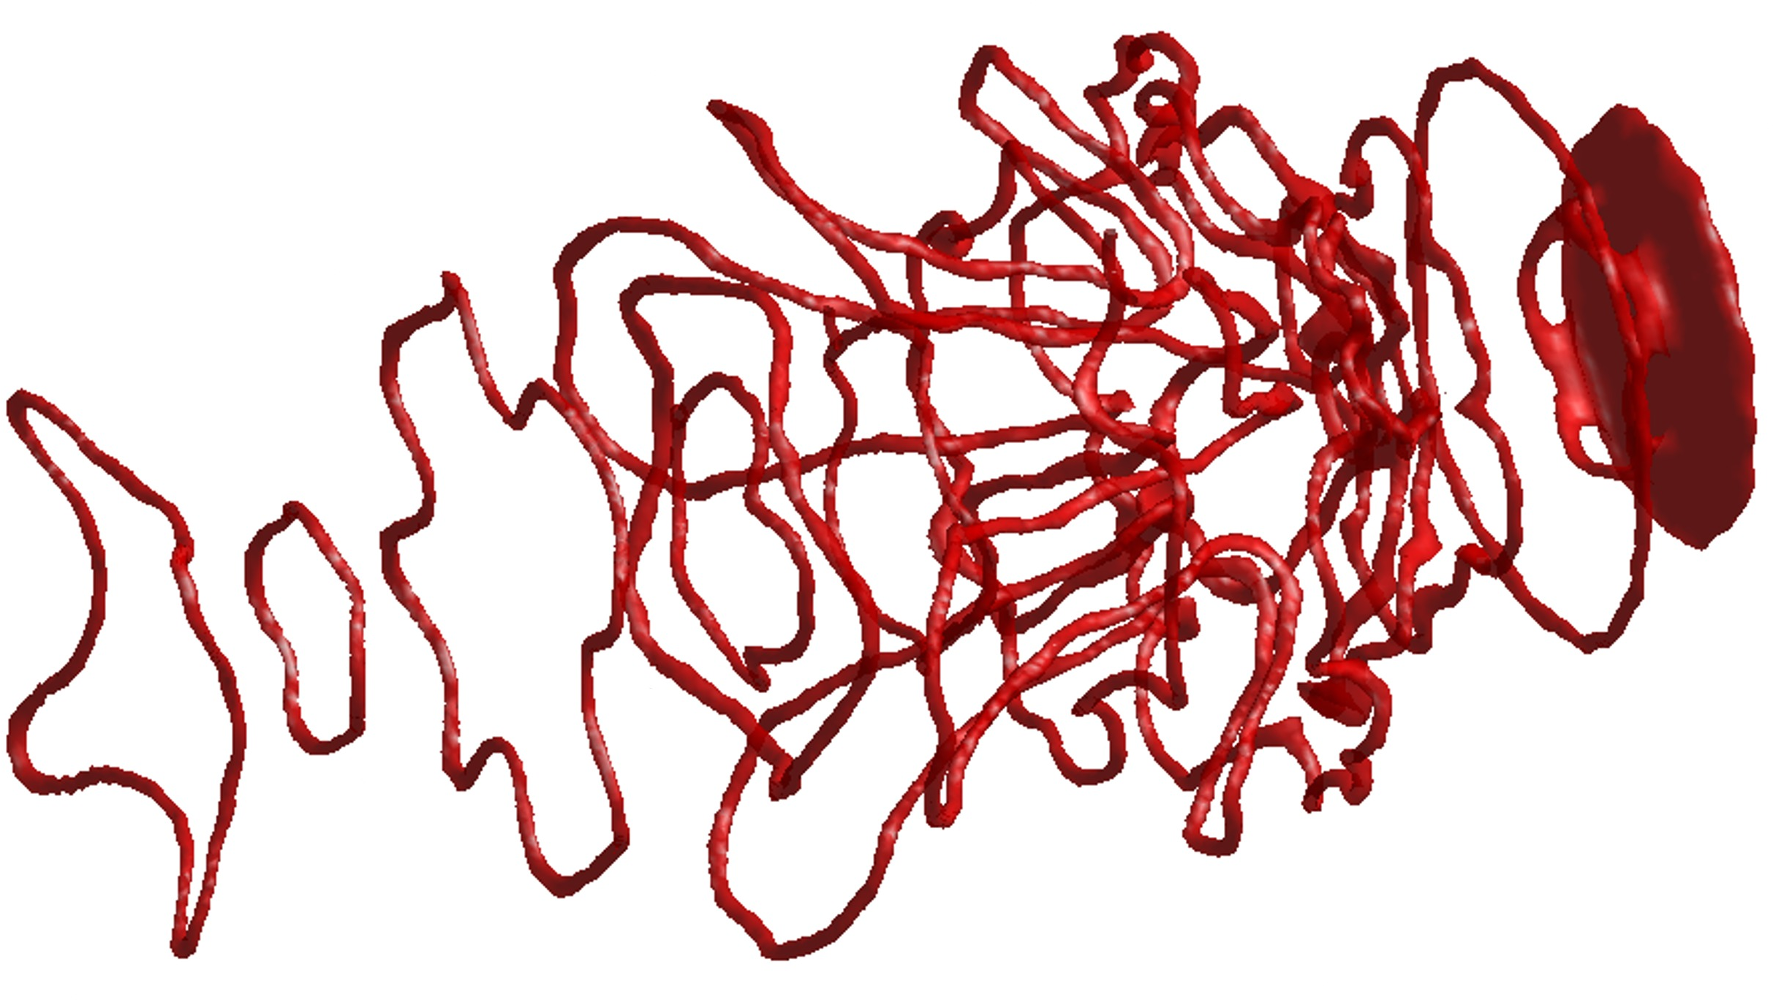
\includegraphics[width=0.9\linewidth]{wake/symwake}
\end{minipage}%
\begin{minipage}{0.5\linewidth}%
\vspace{-0.84\baselineskip}(b)\\
\begin{tikzpicture}[domain=-60:100]
  \begin{axis}[xlabel={$x$}, ylabel={$y$},
      xmin=-60,xmax=100,ymin=-35,ymax=35,
      major tick length = 0.07cm,
      width=\linewidth,
      unit vector ratio=1 1 1,
      scatter/classes={ 0={mark=*,blue},1={mark=o,red}},
      xlabel=$x/\xi$,
      ylabel=$y/\xi$,
      mark size = 0.7
      ]
  \draw[fill] (axis cs:86,0) ellipse [x radius= 1.7, y radius=11];
  \addplot[scatter, only marks,mark options={scale=2}, scatter src=\thisrow{class},
        error bars/.cd, y dir=both, x dir=both, y explicit, x explicit]
        table[x=x,y=y] {wake/symwakevort.dat};
  \end{axis}
\end{tikzpicture}\\%
(c)\\%
\begin{tikzpicture}
  \begin{axis}[ylabel near ticks,xlabel near ticks,
      axis on top,
      width=\linewidth,
      xlabel=$x/\xi$,
      ylabel=$z/\xi$,
      unit vector ratio=1 1 1,
      xmin = -60,xmax = 100,ymin = -35,ymax = 35,
      major tick length = 0.07cm,
    ]
    \addplot graphics [xmin = -60,xmax = 100,ymin = -35,ymax = 35] {wake/symwaketraj};
  \end{axis}
\end{tikzpicture}%
\end{minipage}%
\caption{\label{fig:3d1} Symmetric wake in 3D at $t=450~(\xi/c)$ for an elliptical obstacle ($d=5\xi$ and $\varepsilon=5$) moving at $v=0.6\,c$.  (a) Isosurface plot of low density, over a range $[0,100]$ in $x$ and $[-25,25]$ in $y$ and $z$. (b) Vortex locations in the $xy$ plane.  (c) Vortex trajectories in the $xz$ plane.  In (b) and (c) red/blue denotes vortex lines with quanta of circulation $+1/-1$.}
\end{figure}

\subsection{Symmetric Wakes} 
For a spherical ($\varepsilon=1$) object with $d=5\xi$, we find that the critical velocity is $v_c=0.455\pm 0.05\,c$, consistent with $v_c=0.55\,c$ reported in the Eulerian limit ($d \gg \xi$) \cite{win01,winiecki99}.  Making the obstacle ellipsoidal, with the short direction parallel to the flow, reduces the critical velocity, in parallel with our 2D observations.  For example, for $\varepsilon=5$, the critical velocity is reduced to $v_c=0.315 \pm 0.05\,c$.  Figure \ref{fig:3d1}(a) shows the 3D wake generated past this ellipsoidal obstacle ($d=5\xi$ and $\varepsilon = 5$) when moving at super-critical speed $v=0.6\,c$.  Vortex rings, the 3D analogue of vortex-antivortex pairs, are ejected at high frequency (due to the obstacles high ellipticity) in the direction of the flow.  At early times ($t=450~(\xi/c)$ in this case) the vortex configuration maintains cylindrical symmetry about the obstacle's axis, as is clearly visible in the $xy$ and $xz$ planes in Figure \ref{fig:3d1}(b) and (c).  As the vortex rings move downstream they shrink and speed up, returning to the object, sometimes passing through other vortex rings. A similar behaviour is observed \cite{wacks} in the evolution of toroidal bundles of many coaxial vortex rings which leapfrog around each other.  Occasionally a ring will escape this cycle and fall downstream.  These behaviours lead to the formation of an organized symmetric wake behind the obstacle,  the 3D analogue of our 2D observations.  


\subsection{Asymmetric Wakes}

\begin{figure}[!ht]
(a)\\
\begin{minipage}{0.5\linewidth}%
\centering
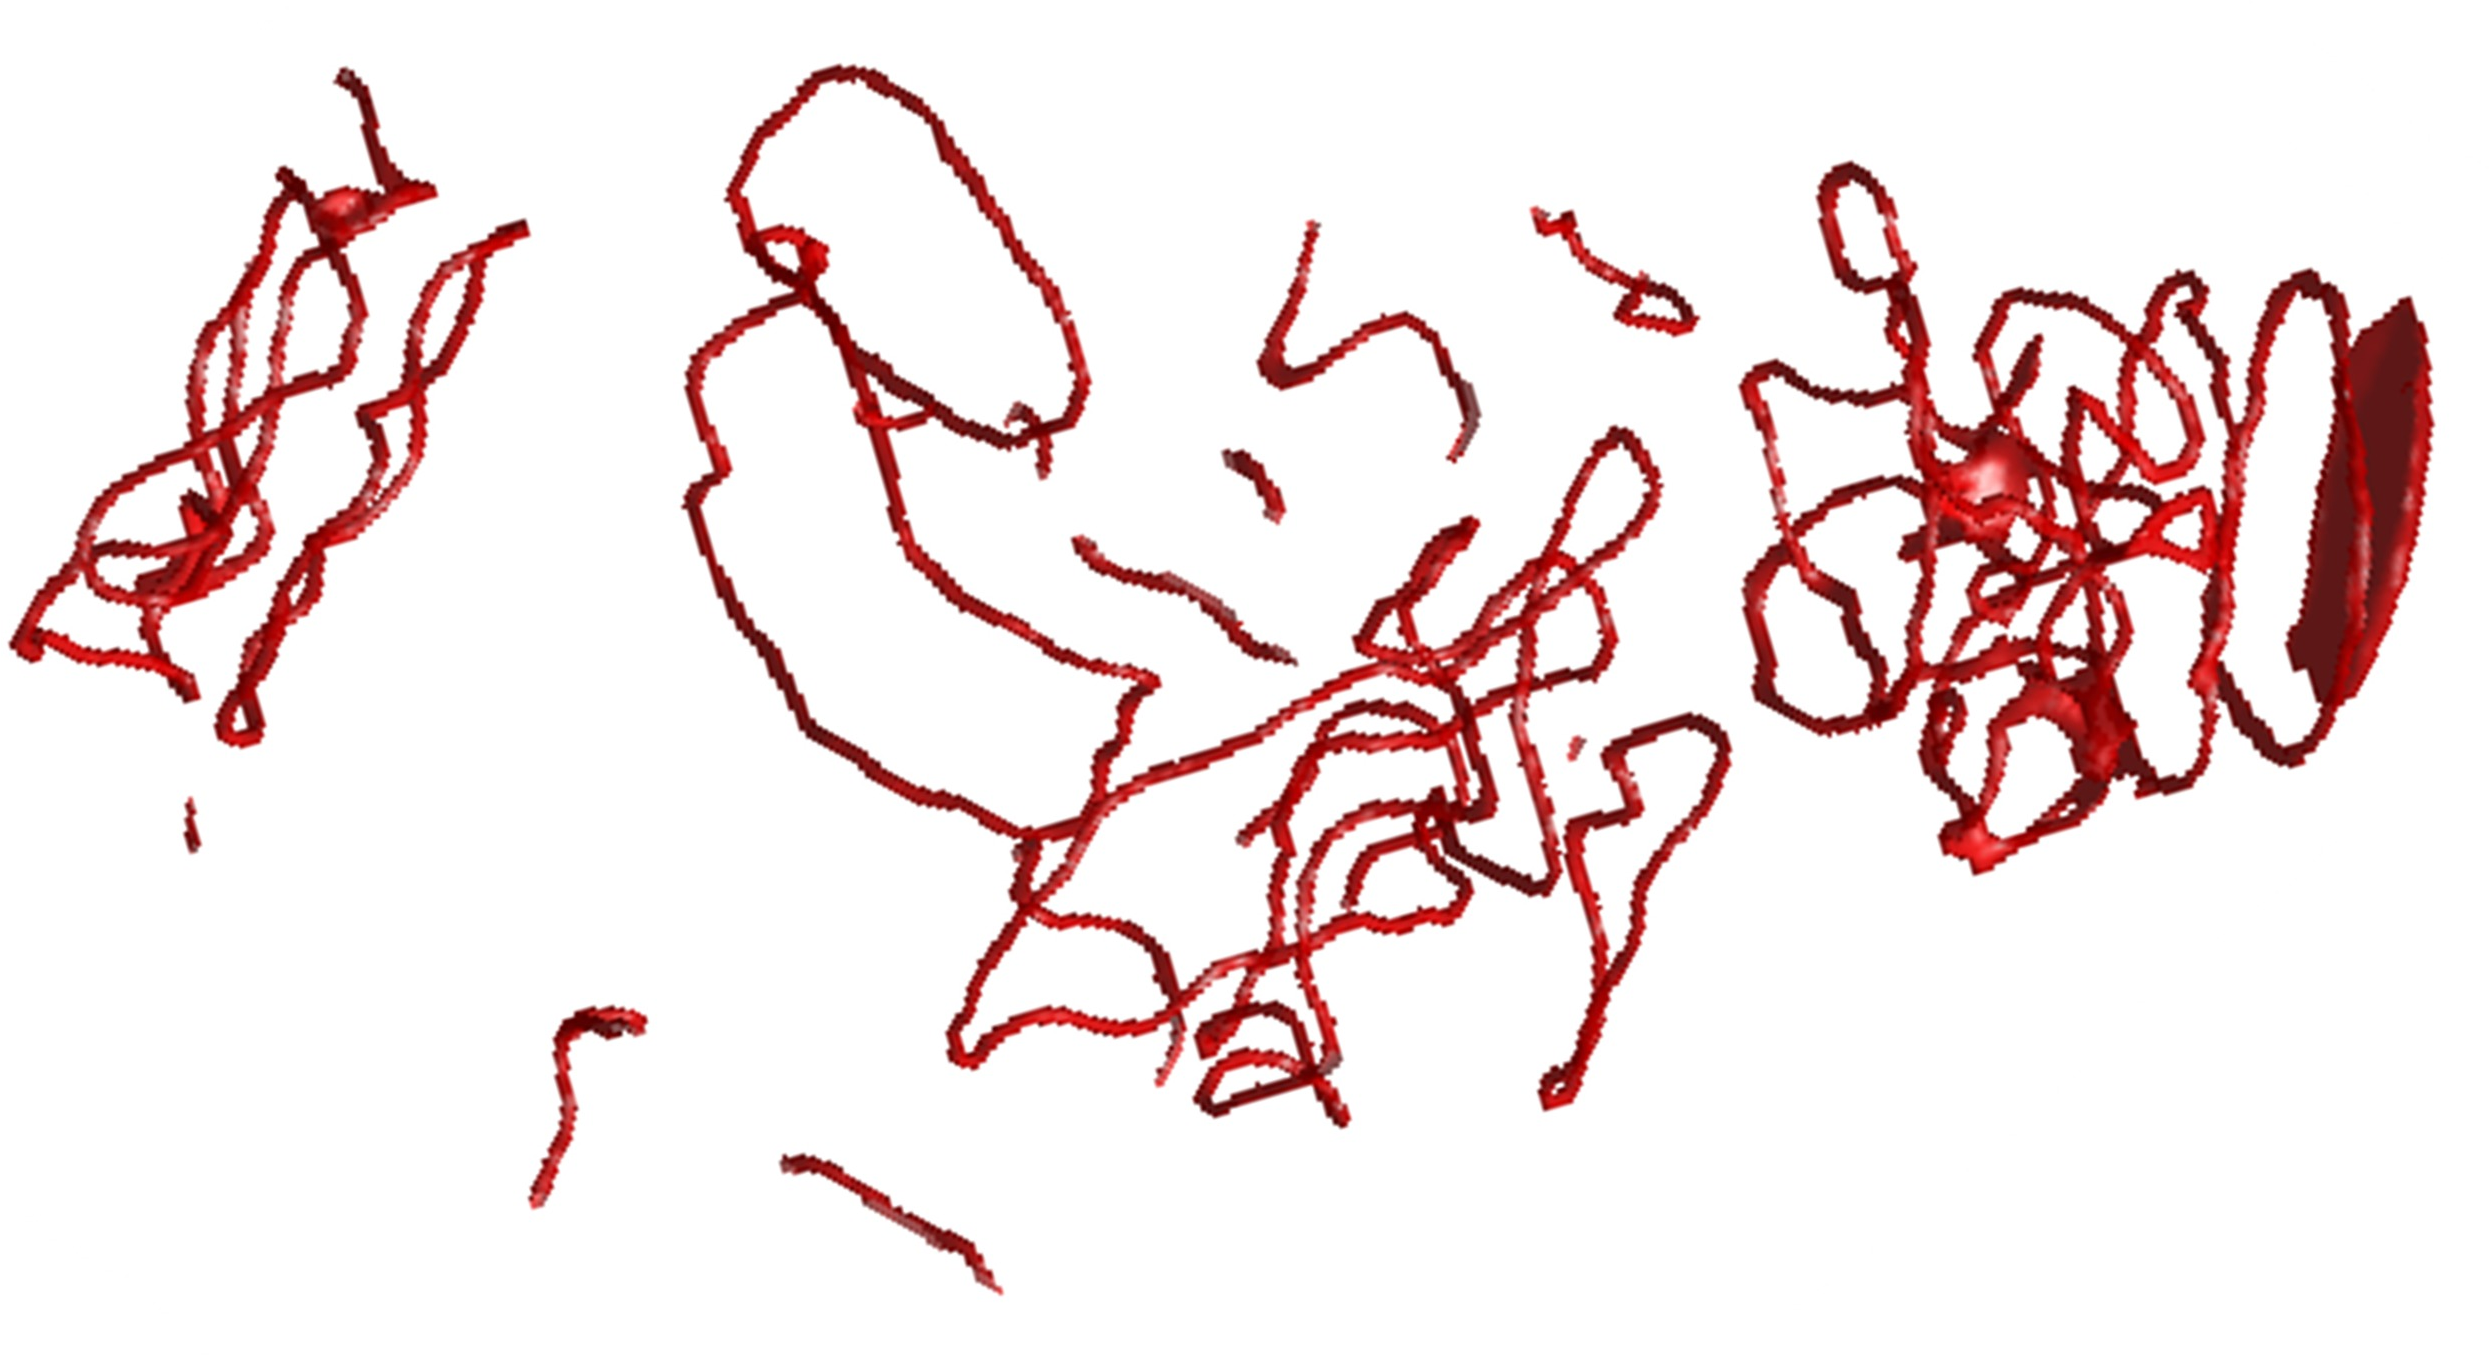
\includegraphics[width=0.9\linewidth]{wake/asymwake}
\end{minipage}%
\begin{minipage}{0.5\linewidth}%
\vspace{-0.84\baselineskip}(b)\\
\begin{tikzpicture}
  \begin{axis}[ylabel near ticks,xlabel near ticks,
      axis on top,
      width=\linewidth,
      xlabel=$x/\xi$,
      ylabel=$y/\xi$,
      unit vector ratio=1 1 1,
      xmin = -60,xmax = 100,ymin = -35,ymax = 35,
      major tick length = 0.07cm,
    ]
    \addplot graphics [xmin = -60,xmax = 100,ymin = -35,ymax = 35] {wake/asymwakeyx};
  \end{axis}
\end{tikzpicture}\\%
(c)\\%
\begin{tikzpicture}
  \begin{axis}[ylabel near ticks,xlabel near ticks,
      axis on top,
      width=\linewidth,
      xlabel=$x/\xi$,
      ylabel=$z/\xi$,
      unit vector ratio=1 1 1,
      xmin = -60,xmax = 100,ymin = -35,ymax = 35,
      major tick length = 0.07cm,
    ]
    \addplot graphics [xmin = -60,xmax = 100,ymin = -35,ymax = 35] {wake/asymwakezx};
  \end{axis}
\end{tikzpicture}%
\end{minipage}%
\caption{\label{fig:3d4} Asymmetric wake in 3D at $t=340~(\xi/c)$ for an elliptical obstacle ($d=5\xi$ and $\varepsilon=5$) moving at $v=0.6\,c$. (a) Isosurface plot of low density, over a range $[-60,100]$ in $x$ and $[-25,25]$ in $y$ and $z$. (b) Vortex locations in the $xy$ plane.  (c) Vortex locations in the $xz$ plane.  In (b) and (c) red/blue denotes vortex lines with quanta of circulation $+1/-1$.}
\end{figure}

We break the cylindrical symmetry of the system by tilting the obstacle by a small angle in the $xz$ plane.  The vortex rings, illustrated in Figure \ref{fig:3d4}, now eject and evolve asymmetrically; Kelvin waves and reconnections occur, forming an apparently disordered tangle of vortices behind the obstacle.  Due to the manner in which symmetry is broken, the wake remains approximately symmetric in the $xy$ plane, as evident in Figure \ref{fig:3d4} (b).  However, unlike in Figure \ref{fig:3d1}, the vortices do not self organise into two clusters of alternate circulation. This is due to the vortex rings interacting, reconnecting and shifting out of the plane (which manifests in 2D as two alternate-sign vortices approaching one another).



However, in the $xz$ plane (Figure \ref{fig:3d4} (c)), symmetry is broken. Due to the relatively high frequency of vortex nucleation and relatively low flow speed, like signed vortices cluster together as they are ejected by the obstacle, much like the 2D solutions seen in earlier sections.  Downstream the tangle may shift both across or out of the plane. In 2D, although this manifests as a shift in location of the vortex clusters, the clusters largely remain rather than forming dipoles. 

\section{Conclusions}
We have shown that the motion of an obstacle in a Bose-Einstein condensate produces classical-like wakes consisting of quantum vortices of the same polarity.  This is consistently observed in both 2D and 3D scenarios.  By modifying the obstacle so that it is elliptical, which reduces the critical velocity for vortex nucleation, vortices are generated at a sufficiently high rate that they undergo strong interactions with their neighbours  (rather than being swept away). This leads to the production of classical-like wakes. Symmetric wakes resemble those observed in classical flow at low $\Rey$.  These are unstable, forming time-dependent asymmetric structures similar to the B\'enard--von K\'arm\'an vortex street of classical fluid dynamics. Vortex singularities
in the inviscid superfluid thus mimic classical vortex patterns typical of viscous flows.  The effects which we describe (dependence of the critical velocity and cluster size on the obstacle's size, velocity and ellipticity) can be experimentally studied in atomic Bose-Einstein condensates using moving laser-induced potentials. They are also relevant to the motion of objects (such as vibrating wires, grids and forks) in superfluid helium, as the obstacle's ellipticity plays a role which is analogous to rough boundaries \cite{blaz08,brad05}. This idea is explored in detail in Chapter \ref{cha:afm}.

\subsection{A `quantum' Reynolds number}
The work in this chapter has been built upon and expanded by Reeves \emph{et. al.} \cite{reeves_2015}. The group performed many 2D simulations using circular ($\varepsilon=1$) Gaussian beams over a large parameter space of $d$ and $v$. By applying the phase unwinding algorithm described in Section \ref{section:vortexremoval} to remove vortices from the periodic flow, the group performed many simulations at efficient resolutions with a high speed GPE numerical simulation GPU/CUDA code running on a cluster of graphics cards. The large number of simulations allowed Reeves \emph{et. al.} to identify a `quantum' Reynolds number, via dynamical similarity of a hard circular cylinder in classical viscous flow and superfluid flow in the presence of a soft Gaussian obstacle.

\end{chapter}
